% Combined hands-on deck, 20 September 2026.
% Sources: rhyme_demo_slides.tex, followed by medea_demo_slides.tex.
\documentclass[aspectratio=169,10pt]{beamer}
\usetheme{metropolis}
% Bundle fonts so XeLaTeX does not depend on operating-system font registration.
\usepackage{fontspec}
\setmainfont{Carlito}[Path=fonts/,Extension=.ttf,UprightFont=*-Regular,BoldFont=*-Bold,ItalicFont=*-Italic,BoldItalicFont=*-BoldItalic]
\setsansfont{Carlito}[Path=fonts/,Extension=.ttf,UprightFont=*-Regular,BoldFont=*-Bold,ItalicFont=*-Italic,BoldItalicFont=*-BoldItalic]
\setmonofont{DejaVuSansMono}[Path=fonts/,Extension=.ttf,UprightFont=*,BoldFont=*-Bold,ItalicFont=*-Oblique,BoldItalicFont=*-BoldOblique,Scale=0.82]
\newfontfamily\porson{GFSPorson.otf}[Path=fonts/]

\usepackage{booktabs,tabularx}
\definecolor{ink}{HTML}{1F2A37}
\definecolor{aegean}{HTML}{5B2C83}
\definecolor{terracotta}{HTML}{B5533C}
\definecolor{olive}{HTML}{5B7F3B}
\definecolor{sand}{HTML}{F4EFE6}
\definecolor{mist}{HTML}{EEE8F4}
\definecolor{slate}{HTML}{6B7A8A}
\setbeamercolor{normal text}{fg=ink,bg=white}
\setbeamercolor{frametitle}{bg=aegean,fg=white}
\setbeamercolor{progress bar}{fg=terracotta,bg=mist}
\setbeamercolor{alerted text}{fg=terracotta}
\setbeamercolor{example text}{fg=olive}
\setbeamercolor{block title}{bg=mist,fg=aegean}
\setbeamercolor{block body}{bg=sand,fg=ink}
\metroset{progressbar=frametitle,block=fill,numbering=fraction}
\setbeamerfont{frametitle}{size=\large,series=\bfseries}
\newcommand{\key}[1]{\textcolor{aegean}{\textbf{#1}}}
\newcommand{\hl}[1]{\textcolor{terracotta}{\textbf{#1}}}
\newcommand{\source}[1]{\vfill{\scriptsize\color{slate}#1\par}}
\newcommand{\observed}{\source{Observed live API run: GPT-4o, 16 September 2026. One run per emotion configuration.}}
\newcommand{\question}[1]{\medskip\par\key{#1}\par}
\newcommand{\emotionlink}{\href{https://greek-app-heaven-medea.livelyhill-85880e66.westeurope.azurecontainerapps.io/emotions}{\textbf{Open Emotion Knowledge Graph}}}
\newcommand{\nesylink}{\href{https://greek-app-heaven-medea.livelyhill-85880e66.westeurope.azurecontainerapps.io/emotions-nesy}{\textbf{Open NeSy Emotions}}}
\newcommand{\zeugmalink}{\href{https://greek-app-heaven-medea.livelyhill-85880e66.westeurope.azurecontainerapps.io/zeugma}{\textbf{Open Zeugma}}}
\newcommand{\thucsource}{Richard Crawley translation, \href{https://github.com/PerseusDL/canonical-greekLit/tree/master/data/tlg0003/tlg001}{Perseus Digital Library, Tufts University}. \href{https://creativecommons.org/licenses/by-sa/4.0/}{CC BY-SA 4.0}.}

\newcommand{\stanza}{%
Πάνω στην άμμο την ξανθή\\[4pt]
γράψαμε τ' όνομά της·\\[4pt]
ωραία που φύσηξεν ο μπάτης\\[4pt]
και σβήστηκε η γραφή.}
\newcommand{\demolink}{\href{https://greek-app-heaven-rhyme.livelyhill-85880e66.westeurope.azurecontainerapps.io}{\textbf{Open Greek Rhyme System}}}

\hypersetup{pdftitle={CLARIN:EL hands-on: rhyme and language analysis applications},pdfauthor={Stergios Chatzikyriakidis}}
\begin{document}


\begin{frame}{1. Try Few-Shot first}
  \begin{columns}[T]
    \begin{column}{0.58\textwidth}
      \begin{block}{Paste this stanza}
        \large\stanza
      \end{block}
      \footnotesize Giorgos Seferis, \emph{Denial}, stanza 2.
    \end{column}
    \begin{column}{0.38\textwidth}
      \textbf{Identification settings}
      \begin{itemize}
        \item Strategy: \key{Few-Shot}
        \item RAG: \hl{OFF}
        \item Verification: \hl{OFF}
      \end{itemize}
      \small Use your own API key or the key supplied for today. Keep the same model for every run.\\[6pt]
      Select \textbf{Ανάλυση} (Analyze).
    \end{column}
  \end{columns}
  \vfill
  \small\demolink\hfill Work in pairs. Save the answer.
  \vspace{3pt}
  \par\footnotesize Verification is on by default: untick it before this first run.
\end{frame}

\begin{frame}{2. ``No need for symbolic rules?''}
  \centering
  {\Large Did Few-Shot get these right?\par}
  \vspace{1em}
  \begin{tabular}{lll}
    \toprule
    \textbf{Lines} & \textbf{Pair} & \textbf{Check for} \\
    \midrule
    1 and 4 & ξανθή / γραφή & M, IDV \\[7pt]
    2 and 3 & όνομά της / μπάτης & \key{F2, MOS} \\
    \bottomrule
  \end{tabular}
  \vspace{1em}
  \begin{block}{If it found the mosaic rhyme\ldots}
    \centering\large ``There you go. Why do we need symbolic verification?''
  \end{block}
  \vspace{0.6em}
  \large Would you trust it on another poem?
\end{frame}

\begin{frame}{3. The answer was already in the prompt}
  \setlength{\parskip}{0pt}
  \begin{block}{Actual excerpt from the Few-Shot prompt}
    \normalsize\ttfamily\raggedright\setlength{\parskip}{0pt}
    \vspace{3pt}
    EXAMPLE 2 - Feminine-2 Mosaic:\par\medskip
    Line 6: "γράψαμε τ' όνομά της" ['Gra-psa-me 'to-no-'ma tis]\par
    Line 7: "ωραία που φύσηξεν ο μπάτης" [o-'re-a pu 'fi-si-ksen o 'ba-tis]\par\medskip
    → Classification: \textcolor{aegean}{\textbf{F2-MOS}}\par\medskip
    [...]\par
    - Rhyme spans word boundary in L6 → MOS
  \end{block}
  \small The same pair, its label and its explanation were supplied as a worked example.\par
  \vspace{0.5em}
  \key{Success here does not establish generalisation to an unseen example.}\par
  \vfill
  \scriptsize Source: \texttt{greek-rhyme/prompts.py}, \texttt{FEW\_SHOT}, Example 2. Its line numbers refer to the original poem.
\end{frame}

\begin{frame}{4. Now remove the worked examples}
  \begin{columns}[T]
    \begin{column}{0.55\textwidth}
      \begin{block}{Same stanza, same model}
        \normalsize\stanza
      \end{block}
      \small Select \textbf{Ανάλυση} again. Save this answer too.
    \end{column}
    \begin{column}{0.41\textwidth}
      \textbf{Change the strategy}
      \begin{itemize}
        \item \key{Zero-Shot Structured}
        \item RAG: \hl{OFF}
        \item Verification: \hl{OFF}
      \end{itemize}
      \small This prompt gives the taxonomy and procedure, without the worked examples.\par
      \vspace{0.7em}
      \textbf{Inspect the difference}\par
      Does it still find \key{F2-MOS}?\par
      Look for a missed mosaic label, a stress error or an invented feature.
    \end{column}
  \end{columns}
  \vfill
  \small Judge the returned answer against the stanza.
\end{frame}

\begin{frame}{5. Switch on phonological verification}
  \small Keep \textbf{Zero-Shot Structured}, the same model and \textbf{RAG OFF}.\\
  Turn \key{Verification ON}, then select \textbf{Ανάλυση}.
  \vspace{0.8em}
  \begin{columns}[T]
    \begin{column}{0.48\textwidth}
      \begin{block}{The rule-based analysis}
        \small ξανθή / γραφή\\[3pt]
        \key{M, IDV}\\[9pt]
        όνομά της / μπάτης\\[3pt]
        \key{F2, MOSAIC}
      \end{block}
      \footnotesize The rhyme domain crosses the boundary in \textbf{μά | της}. The stressed vowel and following sounds match those in \textbf{μπάτης}.
    \end{column}
    \begin{column}{0.48\textwidth}
      \textbf{Read the three output sections}
      \begin{enumerate}
        \item \textbf{INITIAL LLM ANALYSIS}\\What does the model claim?
        \item \textbf{PHONOLOGICAL VERIFICATION}\\What do the rules find?
        \item \textbf{LLM REFLECTION \& CORRECTION}\\Did the model use the report to correct its answer?
      \end{enumerate}
    \end{column}
  \end{columns}
  \vfill
  \small A supplied example can guide an answer. A symbolic check supplies explicit evidence.
\end{frame}




% 1
\begin{frame}{Theory, rules and historical queries}
  \par
  {\LARGE What changes when we make our assumptions explicit?\par}
  \vspace{1em}
  \begin{columns}[T]
    \begin{column}{.31\textwidth}
      \begin{block}{1. Theory in the prompt}
        Cairns-inspired emotion scripts: situation, appraisal and response.
      \end{block}
    \end{column}
    \begin{column}{.31\textwidth}
      \begin{block}{2. Theory in rules}
        Four NeSy modes: inspect an inference, a correction or a disagreement.
      \end{block}
    \end{column}
    \begin{column}{.31\textwidth}
      \begin{block}{3. Query the account}
        Zeugma: extract historical claims, then ask what follows.
      \end{block}
    \end{column}
  \end{columns}
  \medskip
  \small\url{https://stergioscha.github.io/svarna/demos.html}
  \source{Stergios Chatzikyriakidis, ILSP \enspace|\enspace CLARIN:EL, 24 September 2026\\
  Hands-on module. Saved rehearsal outputs are shown after each activity.}
\end{frame}

% 2
\begin{frame}{Achilles puts away the sword. What happens to his anger?}
  \small Homer, \emph{Iliad} 1.172 to 1.224, A. T. Murray's English translation.
  \begin{columns}[T]
    \begin{column}{.48\textwidth}
      \begin{block}{The threat}
        “I will myself come to your tent and take the fair-cheeked Briseis, your prize”
      \end{block}
      \begin{block}{Achilles' response}
        “Grief came upon the son of Peleus”\\[4pt]
        “whether he should draw his sharp sword”
      \end{block}
    \end{column}
    \begin{column}{.48\textwidth}
      \begin{block}{Athene intervenes}
        “But refrain, and obey us.”
      \end{block}
      \begin{block}{The ending}
        “and in no way ceased from his wrath”
      \end{block}
    \end{column}
  \end{columns}
  \question{Distinguish the emotion, the intended action and the completed action.}
  \source{Use the complete passage in the appendix or \texttt{medea\_cairns\_passage\_en.txt}.\\
  Murray, 1924--1925, Perseus, public-domain translation. Quotations are excerpts.}
\end{frame}

% 3
\begin{frame}{Run the same passage with and without the Cairns prompt}
  \emotionlink
  \begin{columns}[T]
    \begin{column}{.47\textwidth}
      \begin{block}{Keep these settings}
        \small
        Text Language: \key{English}\\
        Analysis Mode: \key{Comprehensive}\\
        AI Provider: \key{Auto}\\
        Include Negative Emotions: \key{on}
      \end{block}
      \small Paste the complete Iliad passage. Keep the same text and settings for both runs.
    \end{column}
    \begin{column}{.49\textwidth}
      \begin{enumerate}
        \item Leave \textbf{Enable Script-Based Analysis} unticked.
        \item Select \textbf{Analyze Emotions}. Inspect \textbf{Emotions}; save with \textbf{Download JSON}.
        \item Tick \textbf{Enable Script-Based Analysis}, under \textbf{Enhanced Analysis (Cairns Framework)}.
        \item Analyze and save again.
      \end{enumerate}
    \end{column}
  \end{columns}
  \question{What does the second answer make explicit that the first leaves implicit?}
  \source{Rehearsal used the existing proxy through Auto. Logs confirmed GPT-4o; Auto can select differently on a future run.}
\end{frame}

% 4
\begin{frame}{Standard analysis: a plausible ending to question}
  \begin{block}{Returned emotion labels}
    anger \quad grief \quad hatred \quad wonder \quad \hl{relief}
  \end{block}
  \begin{columns}[T]
    \begin{column}{.48\textwidth}
      \begin{block}{The model's relationship claim}
        “Grief is resolved by relief as Athene intervenes and calms Achilles.”
      \end{block}
    \end{column}
    \begin{column}{.48\textwidth}
      \begin{block}{The passage}
        “But the son of Peleus again addressed with violent words the son of Atreus, and in no way ceased from his wrath:”
      \end{block}
    \end{column}
  \end{columns}
  \question{Does obedience establish relief? What evidence would justify that label?}
  \observed
\end{frame}

% 5
\begin{frame}{Cairns: theory changes the structure of the question}
  \begin{block}{Actual opening of the enhanced prompt}
    \small “Analyze this text for emotional content using SCRIPT-BASED REPRESENTATION with METAPHOR DETECTION.”
  \end{block}
  \small
  \begin{tabularx}{\textwidth}{@{}lX@{}}
    \toprule
    \textbf{Script component} & \textbf{Returned analysis of anger}\\
    \midrule
    Eliciting conditions & Insult to honor; threat to possessions\\
    Appraisals & “I have been disrespected”; “My status is challenged”\\
    Action tendencies & Confront; seek revenge; assert dominance\\
    Cultural norms & Anger is justified in defense of honor\\
    \bottomrule
  \end{tabularx}
  \medskip
  \normalsize The prompt also asks for bodily responses, expressive behaviour and moral evaluations.
  \question{Which connections can you defend from the text?}
  \source{Observed enhanced output. Prompt excerpt from the inspected local template, \texttt{medea\_cairns\_prompt.txt}.\\
  This is the app's Cairns-inspired implementation. [VERIFY: exact deployed prompt revision.]}
\end{frame}

% 6
\begin{frame}{Reveal: prompt examples reappear as “textual evidence”}
  \small
  \begin{tabularx}{\textwidth}{@{}Xccc@{}}
    \toprule
    \textbf{Phrase} & \textbf{Prompt example} & \textbf{Returned evidence} & \textbf{In passage}\\
    \midrule
    “Burning with rage” & yes & yes & \hl{no}\\[5pt]
    “Filled with grief” & yes & yes & \hl{no}\\[5pt]
    “Seized by anger” & yes & yes & \hl{no}\\
    \bottomrule
  \end{tabularx}
  \vspace{1em}
  \begin{block}{A richer account still needs evidence}
    The output also supplies tears and increased heart rate.\\
    A script's typical features need not have occurred in this scene.
  \end{block}
  \question{Mark each claim as quoted evidence, interpretation or unsupported addition.}
  \source{Observed enhanced output, checked against the input and local prompt.\\
  The overlap is consistent with prompt-example contamination; this is not a controlled causal experiment.}
\end{frame}

% 7
\begin{frame}{Four groups, four ways of using the theory}
  \nesylink\par\medskip
  \small
  \begin{tabularx}{\textwidth}{@{}lXX@{}}
    \toprule
    \textbf{Mode} & \textbf{Mechanism} & \textbf{Inspect}\\
    \midrule
    Cairns NeSy1 & Heuristic rules and feedback & A rule and its proposed correction\\
    Cairns NeSy2 & pyDatalog rules and inference & The premises supporting an inference\\
    Cairns NeSy3 & Explicit emotion families and action concepts & What the vocabulary admits or misses\\
    Cairns NeSy4 & Model/grammar dialogue and a critic & A defended reading or proposed amendment\\
    \bottomrule
  \end{tabularx}
  \medskip
  Same Iliad passage. \textbf{Genre Context: Epic}; \textbf{Language: English}; \textbf{AI Provider: Auto}.\\
  Leave \textbf{Enable Feedback Loop} on. Select your mode, then \textbf{Analyze (Neuro-Symbolic)}.
  \question{One operator per group. Bring back one claim, its evidence and your verdict.}
  \source{NeSy3 is selected by default. Choose the assigned mode explicitly. Save with Download JSON.}
\end{frame}

% 8
\begin{frame}{NeSy1: follow a correction all the way back to the text}
  \begin{columns}[T]
    \begin{column}{.59\textwidth}
      \begin{block}{1. The passage}
        “Grief came upon the son of Peleus”
      \end{block}
      \begin{block}{2. The rule's objection}
        “Expected co-occurring 'fear' not found for 'grief'”
      \end{block}
      \begin{block}{3. The feedback result}
        The entity labelled \hl{grief} becomes \hl{anger}.\\
        The feedback item is marked \textbf{resolved}.
      \end{block}
    \end{column}
    \begin{column}{.37\textwidth}
      \textbf{Observed trace}\\[6pt]
      10 entries\\
      6 fired rules\\
      4 inconsistency records\\
      4 feedback calls
      \medskip\par
      \small The feedback discusses Agamemnon, although the target grief belongs to Achilles.
    \end{column}
  \end{columns}
  \question{Was a missing emotion found, or did the feedback replace a supported label?}
  \observed
\end{frame}

% 9
\begin{frame}{NeSy2: inspect the premise as well as the inference}
  \small
  \begin{tabularx}{\textwidth}{@{}Xl@{}}
    \toprule
    \textbf{Rule or check in the returned trace} & \textbf{Observed result}\\
    \midrule
    Anger alongside grief & Dependency satisfied\\[5pt]
    Anger deepens grief & Causal rule fired\\[5pt]
    Grief requires co-occurring fear & Missing dependency\\[5pt]
    Anger requires a hubris-family item & Missing dependency\\
    \bottomrule
  \end{tabularx}
  \medskip
  \begin{block}{After two feedback calls}
    The grief entity is again relabelled \hl{anger}.\\
    Four trace entries, two fired rules, two inconsistency records.
  \end{block}
  \question{Does grief without fear contradict this passage, or challenge the rule?}
  \observed
\end{frame}

% 10
\begin{frame}{NeSy3: what does a clean grammar result establish?}
  \begin{columns}[T]
    \begin{column}{.48\textwidth}
      \begin{block}{Returned labels}
        wrath\\
        grief\\
        indignation\\
        helplessness
      \end{block}
    \end{column}
    \begin{column}{.48\textwidth}
      \begin{block}{Returned checks}
        Grammar compliance: \key{1.0}\\
        Rule firings: \key{0}\\
        Inconsistencies: \key{0}\\
        Symbolic corrections: \key{0}
      \end{block}
    \end{column}
  \end{columns}
  \medskip
  The passage explicitly says: “Achilles was seized with \hl{wonder}”.\\
  Wonder is missing from this constrained extraction.
  \question{What can fall outside the vocabulary while everything inside it passes?}
  \observed
\end{frame}

% 11
\begin{frame}{NeSy4: the model can challenge the grammar}
  \begin{block}{The unconstrained reading adds wonder}
    “Achilles was seized with wonder, and turned around, and immediately recognized Pallas Athene.”
  \end{block}
  \begin{columns}[T]
    \begin{column}{.48\textwidth}
      \begin{block}{Dialogue: defend}
        “The passage explicitly states that Achilles was 'seized with wonder,' which directly supports the proposed emotion of wonder”
      \end{block}
    \end{column}
    \begin{column}{.48\textwidth}
      \begin{block}{Proposed ontology amendment}
        Type: \textbf{new family}\\
        Proposed name: \key{wonder}\\
        Evidence: the quoted passage
      \end{block}
      \small A proposal for human review. It was not applied.
    \end{column}
  \end{columns}
  \question{Would you extend the grammar, revise the label, or defend its existing scope?}
  \source{Observed NeSy4 output. Defence quoted in part. Six dialogue turns, all defend; four amendment proposals.}
\end{frame}

% 12
\begin{frame}{NeSy4: fitting the vocabulary can also change the reading}
  \small Open \textbf{Dialogue (NeSy4)} and compare the free reading with the critic.
  \begin{columns}[T]
    \begin{column}{.48\textwidth}
      \begin{block}{Care becomes pity}
        Passage: Hera “loved and cared for both men alike”.\\[7pt]
        Free reading: \key{care}\\
        Critic revision: \hl{pity}
      \end{block}
    \end{column}
    \begin{column}{.48\textwidth}
      \begin{block}{Obedience becomes submission}
        Passage: Achilles obeys while remaining angry.\\[7pt]
        Free reading: \key{obedience}\\
        Critic revision: \hl{submission}\\
        Assigned family: \textbf{helplessness}
      \end{block}
    \end{column}
  \end{columns}
  \question{Do these revisions preserve what you want to say about the scene?}
  \small The main four-emotion result remains the baseline. Dialogue, critic revisions and amendment proposals are separate outputs.
  \observed
\end{frame}

% 13
\begin{frame}{Zeugma: extract the Theban entry into Plataea}
  \zeugmalink
  \begin{columns}[T]
    \begin{column}{.48\textwidth}
      \begin{block}{Thucydides 2.2}
        Theban troops enter Plataea at night.\\[5pt]
        Naucleides opens the gates.\\[5pt]
        The intruders make a proclamation, hoping the city will join them.
      \end{block}
      \footnotesize Scene summary. The verbatim selection and queries are together in the appendix; the saved graph follows this slide.
    \end{column}
    \begin{column}{.48\textwidth}
      \begin{enumerate}
        \item Paste the text under \textbf{Step 1: Ancient Text for Graph Extraction}.
        \item Keep \textbf{Reasoning Mode: Basic - General logical reasoning} and the same provider.
        \item Select \textbf{Step 1: Extract Knowledge Graph}.
        \item Inspect \textbf{Available Predicates}.
      \end{enumerate}
    \end{column}
  \end{columns}
  \question{Find one actor, one place and one relationship that the passage supports.}
  \source{One shared extraction for the room. Source text: \texttt{medea\_zeugma\_passage\_short\_en.txt}.\\
  \thucsource}
\end{frame}

% 14
\begin{frame}{The saved graph used for the six queries}
  \small Shorter Thucydides selection: \textbf{9 entities, 11 relations}.
  {\centering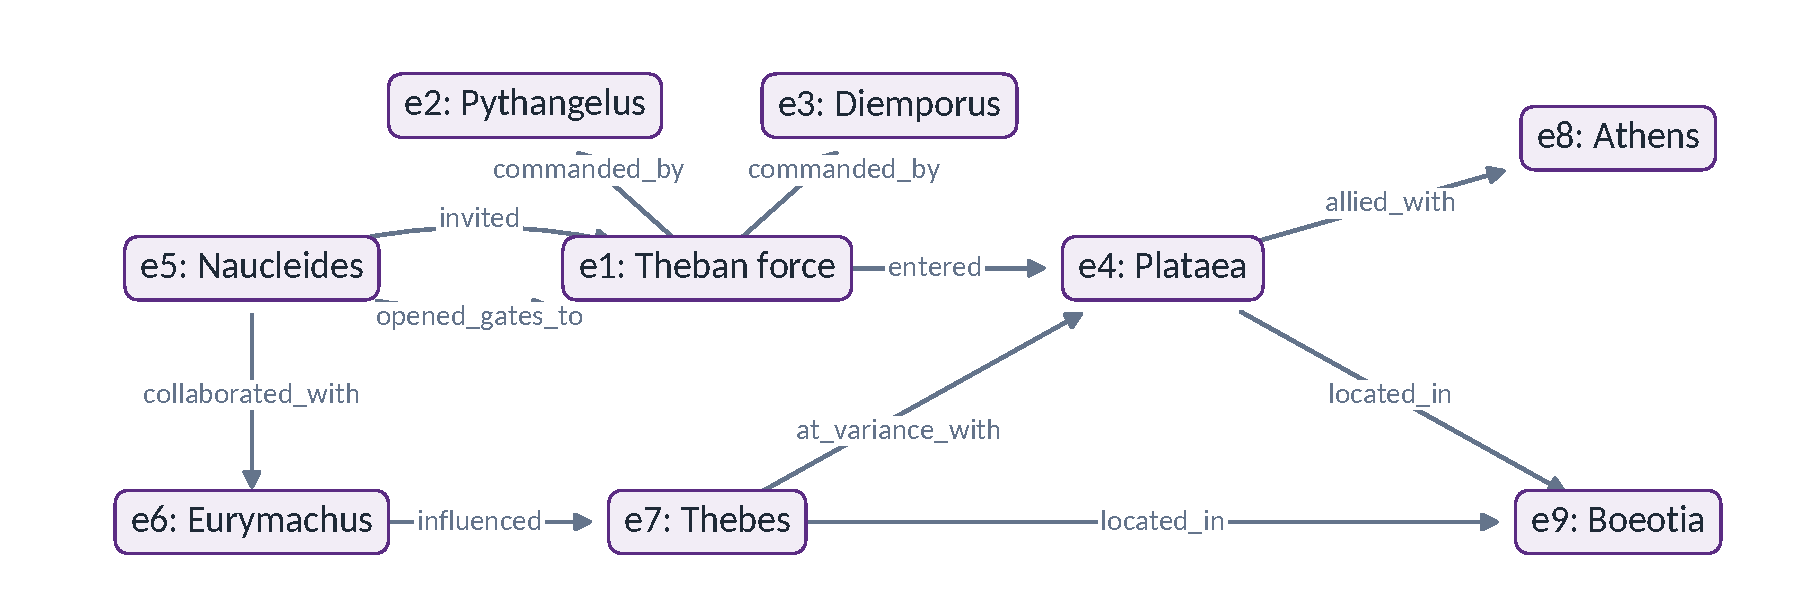
\includegraphics[width=\textwidth,height=.56\textheight,keepaspectratio]{zeugma_materials/short_graph.pdf}\par}
  \footnotesize The diagram preserves the returned \texttt{allied\_with} edge. The successful query uses the literal property \texttt{alliance(e4, 'Athens')}.
  \source{Drawn from the saved API response, 16 September. Every returned entity and relation is shown.\newline
  Exact facts, source text and query answers: \texttt{zeugma\_materials.pdf}. IDs belong to this extraction.}
\end{frame}

\begin{frame}{Ask a question, then follow the shared variable}
  \small Under \textbf{Step 2: Zeugma Symbolic Queries}, enter one complete query per line.\\
  Select \textbf{Run Queries}.
  \begin{block}{Who commanded the force?}
    \small\ttfamily\raggedright\setlength{\parskip}{0pt}
    commanded\_by(Force, Commander),\par
    entity(Commander, Name, person)
  \end{block}
  \small Observed: \key{Pythangelus} and \key{Diemporus}.
  \begin{block}{Who opened the gates to a force entering which city?}
    \small\ttfamily\raggedright\setlength{\parskip}{0pt}
    opened\_gates\_to(Person, Force), entered(Force, Place),\par
    entity(Person, Name, person), entity(Place, City, place)
  \end{block}
  \small Observed: \key{Naucleides}, \key{Plataea}.
  \question{The repeated variable connects the facts. Are those facts supported?}
  \source{Queries wrap visually here; paste each query as one line. Names and IDs may change after a fresh extraction.}
\end{frame}

% 15
\begin{frame}{The saved graph behind the historical-error discussion}
  \small \textbf{Separate run: full Thucydides 2.2.} These are its four disputed edges.
  {\centering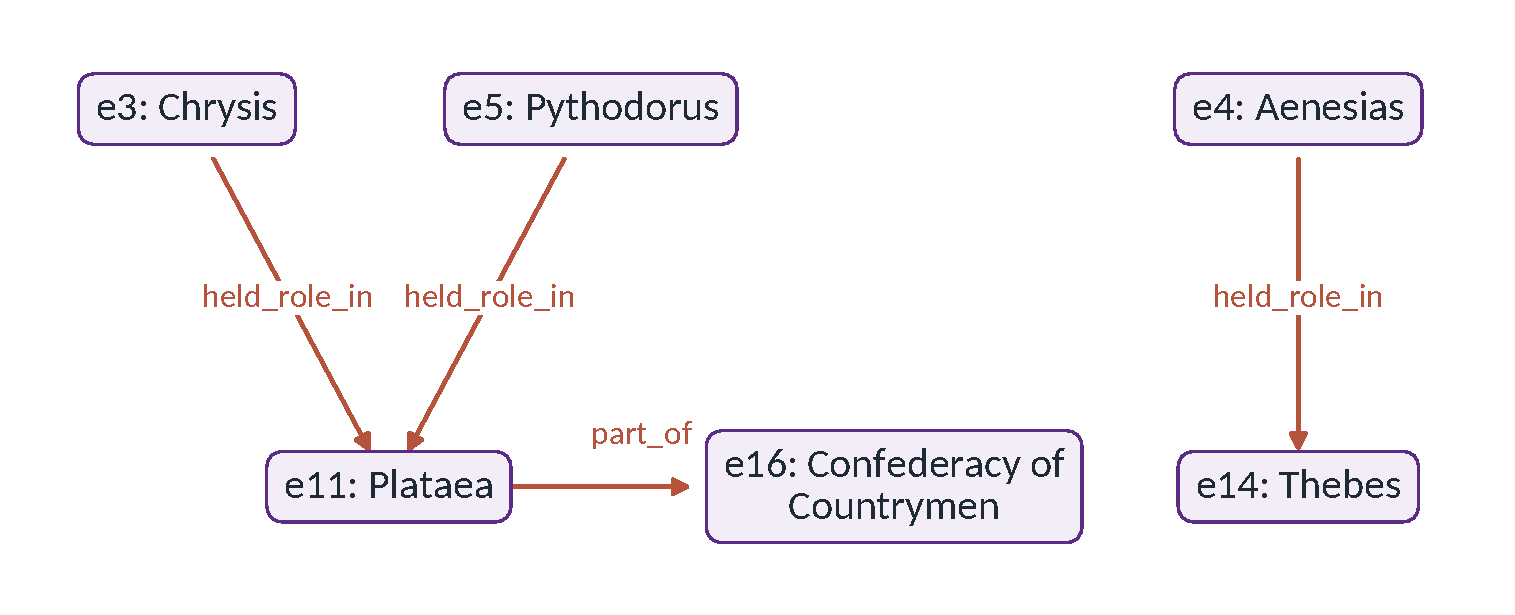
\includegraphics[width=\textwidth,height=.58\textheight,keepaspectratio]{zeugma_materials/focus_graph.pdf}\par}
  \small Read the arrows as the model's assertions. Compare them with the source text on the next slide.
  \source{Exact IDs and predicates from the saved full-passage response. This is a selected subgraph.\newline
  The complete 16-entity, 14-relation graph is in the appendix and \texttt{zeugma\_materials.pdf}.}
\end{frame}

\begin{frame}{The graph turns an invitation into an established fact}
  \small Saved extraction from the \textbf{full} Thucydides 2.2 passage.
  \begin{columns}[T]
    \begin{column}{.56\textwidth}
      \begin{block}{An invitation becomes membership}
        \textbf{Text:} The herald invites Plataea to join the confederacy. The Thebans hope it will join.\\[6pt]
        \textbf{Graph:} Plataea \hl{is part of} the confederacy (\texttt{part\_of}).
      \end{block}
      \key{The text never reports acceptance.}
    \end{column}
    \begin{column}{.40\textwidth}
      \begin{block}{Other errors: office locations}
        \footnotesize
        \begin{tabular}{@{}lll@{}}
          \toprule
          \textbf{Person} & \textbf{Text} & \textbf{Graph}\\
          \midrule
          Chrysis & Argos & \hl{Plataea}\\[3pt]
          Aenesias & Sparta & \hl{Thebes}\\[3pt]
          Pythodorus & Athens & \hl{Plataea}\\
          \bottomrule
        \end{tabular}\\[4pt]
        Graph predicate: \texttt{held\_role\_in}.
      \end{block}
    \end{column}
  \end{columns}
  \medskip
  \textbf{Why the check misses these errors:} it checks that the linked entities exist.\\
  It reports consistency \textbf{1.0} and zero contradictions without checking textual support.
  \question{Correct reasoning over this graph can still give a wrong historical answer.}
  \source{Observed full-passage extraction. The current UI does not run the separate paper's historical validation workflow.}
\end{frame}

% 16
\begin{frame}{When a query returns nothing, check what failed}
  \begin{columns}[T]
    \begin{column}{.48\textwidth}
      \begin{block}{The full passage}
        The apostrophe in \textbf{Thirty Years' Truce} broke the generated Prolog.\\[7pt]
        Seven of eight queries returned no solutions.
      \end{block}
      \small The page had reported successful extraction.
    \end{column}
    \begin{column}{.48\textwidth}
      \begin{block}{The shorter passage}
        Five of six initial queries worked.\\[7pt]
        An alliance rule failed; the direct \textbf{alliance} property worked.
      \end{block}
      \small All six revised classroom queries have successful rehearsal records.
    \end{column}
  \end{columns}
  \question{A missing fact, a wrong representation, or an execution error?}
  \small Use the tested selection and inspect \textbf{Detailed Output Log}. Keep the source passage beside the results.
  \source{Input/query workarounds only. The existing app was not changed. Both returned RDF exports also failed a local Turtle syntax check.}
\end{frame}

% 17
\begin{frame}{Bring back one claim you can defend}
  \begin{columns}[T]
    \begin{column}{.31\textwidth}
      \begin{block}{Prompt}
        Which theoretical distinction made the reading more precise?\\[8pt]
        Which added detail lacked evidence?
      \end{block}
    \end{column}
    \begin{column}{.31\textwidth}
      \begin{block}{Rules}
        Which premise supported the inference?\\[8pt]
        Which “correction” would you reject?
      \end{block}
    \end{column}
    \begin{column}{.31\textwidth}
      \begin{block}{Queries}
        Which answer followed from the graph?\\[8pt]
        What must still be checked against the source?
      \end{block}
    \end{column}
  \end{columns}
  \vspace{1em}
  {\large\key{Your contribution: a claim, its textual evidence, and the assumption it depends on.}\par}
  \source{The apps remain available after the session: \url{https://stergioscha.github.io/svarna/demos.html}\newline Funding from Microsoft's LINGUA project supported CoDAG (Computational Dialectal Atlas of Greek), making Svarna, GPT-4.1 fine-tuning and the Greek NLP Swiss Knife possible.}
\end{frame}


% Nature Analysis extension, proposed exercise, not a saved model result.
\begin{frame}{Nature Analysis: interpretation through an LLM}
  \href{https://greek-app-heaven-nature.livelyhill-85880e66.westeurope.azurecontainerapps.io}{\textbf{Open Nature Analysis}}\par\medskip
  \begin{columns}[T]
    \begin{column}{.48\textwidth}
      \begin{block}{What the model supplies}
        Flora, fauna, sea, land and weather.\\[5pt]
        Metaphor, personification, emotional tone and attitudes towards nature.
      \end{block}
    \end{column}
    \begin{column}{.48\textwidth}
      \begin{block}{What the application adds}
        Segmentation, filtering, counts and exports.\\[5pt]
        \hl{No independent symbolic verifier.}
      \end{block}
    \end{column}
  \end{columns}
  \question{What counts as nature: a physical setting, a metaphor, or a memory?}
  \small Choose the original teaching passage or the Papadiamantis story introduced below.
  \source{Whole Text tested live with Claude Sonnet 5, 20 September 2026. Model output still needs interpretation.}
\end{frame}

\begin{frame}{Run the Greek passage paragraph by paragraph}
  \begin{columns}[T]
    \begin{column}{.48\textwidth}
      \begin{block}{Input and settings}
        File: \texttt{nature\_excerpt.txt}\\[5pt]
        Segmentation: \key{Paragraphs}\\
        Minimum words: \key{20}\\
        Nature threshold: \key{0.2}
      \end{block}
      \small Keep all five paragraphs. The full text is reproduced in the appendix.
    \end{column}
    \begin{column}{.48\textwidth}
      \begin{enumerate}
        \item Use the existing login and your own or supplied provider key.
        \item Paste under \textbf{Paste your text here:}.
        \item Select the provider and model, then \textbf{Analyze Nature Content}.
        \item Save with \textbf{Export JSON} or \textbf{Export CSV}.
      \end{enumerate}
    \end{column}
  \end{columns}
  \question{Before running it, decide what you would count in each paragraph.}
  \source{Original fictional passage written for this exercise, not attributed to a published author.\\
  Whole Text tested with Claude Sonnet 5. [VERIFY: paragraph comparison.]}
\end{frame}

\begin{frame}{Five paragraphs, five annotation decisions}
  \small
  \begin{tabularx}{\textwidth}{@{}lXX@{}}
    \toprule
    \textbf{Part} & \textbf{Evidence in the text} & \textbf{Decision to discuss}\\
    \midrule
    1 & Coast, trees, gull, wind and rain & Which elements are literally present?\\[4pt]
    2 & Office, application and contract & Does the surrounding landscape affect this label?\\[4pt]
    3 & “θύελλα αντιδράσεων”, “βαθιές ρίζες” & Are metaphors counted as weather or flora?\\[4pt]
    4 & Angry sea, absent reeds, remembered frogs & Mention, present entity or remembered environment?\\[4pt]
    5 & Chapel, olive trees, labour and memory & Does a religious gesture establish a religious attitude towards nature?\\
    \bottomrule
  \end{tabularx}
  \question{Declare the annotation policy before judging the model.}
  \source{Questions grounded in the teaching passage. These are not observed model errors.}
\end{frame}

\begin{frame}{Change the unit, then inspect the statistic}
  \small Save the first result. Change only \textbf{Segmentation} to \textbf{Whole Text} and rerun.
  \begin{block}{What the nature percentage counts}
    Successful segments above the nature threshold, divided by all successfully analysed segments.
  \end{block}
  \begin{columns}[T]
    \begin{column}{.48\textwidth}
      \begin{block}{Paragraphs}
        Several separate judgements.\\
        The administrative paragraph can differ from its neighbours.
      \end{block}
    \end{column}
    \begin{column}{.48\textwidth}
      \begin{block}{Whole Text}
        One judgement for the entire passage.\\
        The percentage now concerns a single segment.
      \end{block}
    \end{column}
  \end{columns}
  \question{Did the interpretation change, the counting unit change, or both?}
  \source{Definition checked in the inspected source. Scores are LLM judgements; they are not independently verified.\\
  Record the model actually used. [VERIFY: observed differences between the two runs.]}
\end{frame}

\begin{frame}{Alternative: Papadiamantis, The Seal's Lament}
  \begin{columns}[T]
    \begin{column}{.48\textwidth}
      \begin{block}{Αλέξανδρος Παπαδιαμάντης}
        {\large\porson Τὸ Μυρολόγι τῆς φώκιας}
      \end{block}
      \small A grandmother washes by the sea. Her granddaughter drowns unheard. A seal finds the child and the narrator gives its lament human words.
      \medskip\par
      Full Greek text: \texttt{papadiamantis\_seal.txt}
    \end{column}
    \begin{column}{.48\textwidth}
      \begin{block}{What to inspect}
        Landscape and animal life.\\[5pt]
        Human lament, flute and sea sounds.\\[5pt]
        The seal as animal and mourner.\\[5pt]
        Seaweed and shells as funeral adornment.
      \end{block}
      {\porson Φύκια ᾽ναι τὰ στεφάνια της,\\
      κοχύλια τὰ προικιά της…}
    \end{column}
  \end{columns}
  \question{Can one tone label capture mourning, pleasure and the animal's feeding?}
  \source{\href{https://www.papadiamantis.net/aleksandros-papadiamantis/syggrafiko-ergo/diigimata/257-t-myrologi-t-s-fokias-1908}{Society for Papadiamantis Studies: complete Greek text}. First published 1908.\\
  For this story use Paragraphs, Minimum words 5. [VERIFY: app output on this story.]}
\end{frame}

% Optional corpus modules. These replace a workshop slot; they do not extend it.
\begin{frame}{Voyant-NLP: can we find the seal?}
  \href{https://greek-app-heaven-voyant.livelyhill-85880e66.westeurope.azurecontainerapps.io}{\textbf{Open Voyant-NLP}}\par\medskip
  \small Paste \texttt{papadiamantis\_seal.txt} under \textbf{Upload}; select \textbf{Add to Corpus}, then \textbf{Concordance}.\par\medskip
  \begin{tabularx}{\textwidth}{@{}lclX@{}}
    \toprule
    \textbf{Search} & \textbf{Matches} & \textbf{Form in the text} & \textbf{What changed?}\\
    \midrule
    φώκια & 0 & & Modern spelling misses the historical form.\\[5pt]
    φώκ & 3 & φώκη, φώκης & A shared fragment finds inflected forms.\\[5pt]
    φωκ & 1 & φωκῶν & The accent falls elsewhere.\\
    \bottomrule
  \end{tabularx}
  \question{Read the contexts: when is the seal feeding, listening or mourning?}
  \small Four explicit word-form matches do not recover every reference to the animal.
  \source{Observed in the live browser, 19 September 2026. Literal substring search; no LLM key needed.}
\end{frame}

\begin{frame}{Voyant-NLP: what does a zero sentiment score mean?}
  \small Open \textbf{Sentiment \& Clusters}, then select \textbf{Analyze} under \textbf{Sentiment Analysis}.
  \begin{columns}[T]
    \begin{column}{.47\textwidth}
      \begin{block}{Observed on the complete story}
        Average polarity: \key{0.0}\\[6pt]
        Average subjectivity: \key{0.0}\\[6pt]
        Every returned segment also scored zero.
      \end{block}
    \end{column}
    \begin{column}{.49\textwidth}
      \begin{block}{Read the text beside the score}
        Bereavement, drowning and lament.\\[6pt]
        Music, pleasure and the animal's meal.\\[6pt]
        Which of these does polarity measure?
      \end{block}
    \end{column}
  \end{columns}
  \question{Does this result establish that the story is emotionally neutral?}
  \source{The inspected source uses default TextBlob sentiment, an English-oriented analyzer, on Greek text.\\
  Corpus statistics and NLP models require language and task checks too.}
\end{frame}

\begin{frame}{Svarna: one marker, different contexts}
  \href{https://greek-corpus-workbench.wonderfulhill-e1c9f1a0.westeurope.azurecontainerapps.io}{\textbf{Open Svarna Greek Corpus Workbench}}\par\medskip
  \small A separate app for existing corpora. Keep the database on \key{corpus}.
  \begin{enumerate}
    \item Open \textbf{Concordancer}; search \key{λοιπόν}.
    \item Select \textbf{europarl} under \textbf{Corpus}, then search.
    \item Repeat with \textbf{opensubtitles}; read beyond the first short rows.
  \end{enumerate}
  \begin{block}{Actual examples}
    Συμφωνούμε, λοιπόν.\quad Παραδεχτείτε το λοιπόν!\\[6pt]
    Λοιπόν;\quad Λοιπόν, λοιπόν, λοιπόν.
  \end{block}
  \question{Inference, transition, an interactional prompt, or insufficient context?}
  \source{A parliamentary source does not guarantee an inferential function. Subtitles are not spontaneous conversation.\\
  Browser searches took about 21--33 seconds in rehearsal. Preload the result pages.}
\end{frame}

\begin{frame}{Svarna dialectal: the same form across varieties}
  \small Change the database selector to \key{dialectal}. Search \key{ίντα}.
  \begin{columns}[T]
    \begin{column}{.48\textwidth}
      \begin{block}{Corpus: grdd\_cretan}
        ίντα μιλείς;\\[8pt]
        και δεν κατέχω, ίντα να πω
      \end{block}
      \small The second quotation is a fragment of a longer verse line.
    \end{column}
    \begin{column}{.48\textwidth}
      \begin{block}{Corpus: grdd\_cypriot}
        Ίντα κλαίεις;\\[8pt]
        Ίντα μμάθκια!!
      \end{block}
      \small Compare the surrounding words and the punctuation.
    \end{column}
  \end{columns}
  \question{A direct question, an embedded question, or an exclamation?}
  \small Does one Modern Greek gloss work in every example? Separate dialect, genre and spelling.
  \source{Both browser searches succeeded, 19 September 2026. A short bridge to the later dialect session.\\
  Collection labels describe the source corpus; they do not verify every word's dialect.}
\end{frame}

\begin{frame}{Svarna LLM: classify a function or explain a pattern}
  \small Open \textbf{LLM}. Select a provider and enter a valid key for that provider.
  \begin{columns}[T]
    \begin{column}{.48\textwidth}
      \begin{block}{Marker Classification}
        Enter \key{λοιπόν}.\\[5pt]
        Select \textbf{Ταξινόμηση} (Classification).\\[5pt]
        Up to 50 retrieved sentences.\\[5pt]
        Function, confidence and a Greek explanation for each sentence.
      \end{block}
    \end{column}
    \begin{column}{.48\textwidth}
      \begin{block}{Pattern Synthesis}
        Enter \key{ίντα}.\\[5pt]
        Select \textbf{Ανάλυση} (Analysis).\\[5pt]
        Up to 30 sentences plus frequency data.\\[5pt]
        An English account of usage, position, functions and variation.
      \end{block}
    \end{column}
  \end{columns}
  \question{Label examples yourself, then check the model's claims against them.}
  \source{Confidence is self-reported. No symbolic checker verifies the linguistic interpretation.\\
  {}[VERIFY: model outputs. The available Gemini credential was rejected in rehearsal.]}
\end{frame}

\begin{frame}{Inspect the evidence that the LLM actually receives}
  \begin{block}{Observed browser input for the ίντα synthesis}
    Database: \key{dialectal}. Concordancer filter: \key{grdd\_cypriot}.\\[5pt]
    Proposed LLM sample: \hl{13 Cretan and 17 Cypriot rows}.
  \end{block}
  \begin{itemize}
    \item The database choice carries through; the individual dialect filter does not.
    \item Sentence text is sent without its individual corpus label.
    \item The frequency table counts matching sentence rows, not every occurrence.
  \end{itemize}
  \question{Which claims about dialect differences can this input support?}
  \small Treat the result as an interpretation of a mixed sample. Return to the source rows before accepting a generalisation.
  \source{Input captured locally before model submission; it is not a generated result.\\
  Source-based prompt templates: \texttt{svarna\_llm\_prompts.md}.}
\end{frame}

\begin{frame}{PlotAnalyzer: one story, different narrative theories}
  \href{https://greek-app-heaven-plot.livelyhill-85880e66.westeurope.azurecontainerapps.io}{\textbf{Open PlotAnalyzer}}\par\medskip
  \begin{columns}[T]
    \begin{column}{.46\textwidth}
      \begin{block}{Keep the input type explicit}
        \small Greek original:\\
        \texttt{papadiamantis\_seal.txt}\\
        Mode: \key{Short Story}\\[8pt]
        English instructor synopsis:\\
        \texttt{plot\_papadiamantis\_synopsis\_en.txt}\\
        Mode: \key{Treatment / Summary}
      \end{block}
    \end{column}
    \begin{column}{.50\textwidth}
      \small
      \begin{enumerate}
        \item Switch \textbf{NeSy} off; leave \textbf{Heuristic} on and the embedding key empty.
        \item \textbf{Import} \texttt{plot\_keyword\_starter.json}.
        \item Paste the full input. Choose Mode, then Theory.
        \item Select \textbf{Analyze Plot}, inspect \textbf{Heuristic}, then \textbf{Export}.
      \end{enumerate}
    \end{column}
  \end{columns}
  \source{Existing UI workaround: Import makes the Heuristic result view accessible. Recompute after importing.\\
  The English synopsis is an instructor adaptation, not a published translation.}
\end{frame}

\begin{frame}{PlotAnalyzer: unavailable data becomes a misleading grade}
  \small Complete Greek story, \textbf{Short Story}, \textbf{Aristotelian (Poetics)}, keyword mode.
  \begin{columns}[T]
    \begin{column}{.47\textwidth}
      \begin{block}{What the dashboard displayed}
        \Large \hl{0\% \quad F \quad Incomplete}
      \end{block}
      \small “0 of 12 elements detected”
    \end{column}
    \begin{column}{.49\textwidth}
      \begin{block}{What the detailed results said}
        Keyword analysis unavailable for non-Latin script.
      \end{block}
      \small All twelve exported feature scores were \key{null}, meaning unavailable.
    \end{column}
  \end{columns}
  \question{Has the story failed the theory, or has the method failed to analyse the text?}
  \small Freytag scored only sentence-length variation; its narrative feature scores were also unavailable.
  \source{Observed live browser runs, 19 September 2026. No model calls.\\
  The displayed grade does not establish a literary judgment or a symbolic validation result.}
\end{frame}

\begin{frame}{PlotAnalyzer: which words produced the score?}
  \small Same English synopsis, \textbf{Treatment / Summary}, keyword mode.\par\medskip
  \footnotesize
  \begin{tabularx}{\textwidth}{@{}lclX@{}}
    \toprule
    \textbf{Feature} & \textbf{Score} & \textbf{Matched words} & \textbf{Check against the input}\\
    \midrule
    Pathos & 37 & mourning, suffering, death & Relevant to the story's suffering.\\[5pt]
    Beginning & 31 & beginning, before & Both concern the seal's late evening meal.\\[5pt]
    Recognition & 13 & who & Relative clauses, not a character's discovery.\\[5pt]
    Framing & 27 & narrator, reader, heard & Read the narrated and translated lament.\\[5pt]
    Defamiliarization & 0 & No matches & What about the seal given a human voice?\\
    \bottomrule
  \end{tabularx}
  \question{A useful lexical clue, a misleading match, or an unsupported absence?}
  \source{First three rows: Aristotelian theory. Last two: Russian Formalism. Actual browser exports.\\
  Scores are keyword formulas; do not rank theories or literary quality by these numbers.}
\end{frame}

\begin{frame}{PlotAnalyzer NeSy: examine the theory inside the rule}
  \small Proposed comparison: Greek original, \textbf{Short Story}, one model, fixed settings.
  \begin{enumerate}
    \item Enable \textbf{NeSy}, enter an OpenRouter key, and switch \textbf{Heuristic} off.
    \item Keep \textbf{Contrastive} off. Compare \textbf{Feedback Loop} off and on.
    \item Save each result. Compare \textbf{Aristotelian (Poetics)} with \textbf{Russian Formalism}.
  \end{enumerate}
  \begin{block}{One rule in the app's Aristotelian schema}
    “Suffering needs Flaw: the error must precede its consequences”
  \end{block}
  \question{Whose error would count? Must this story's suffering require a tragic flaw?}
  \small Also ask who recognizes the drowning: grandmother, reader or seal.
  \source{This is the app's operational rule, not a quotation from Aristotle.\\
  {}[VERIFY: NeSy results and feedback effects. Browser confirmed the OpenRouter key requirement; no key was available.]}
\end{frame}

\begin{frame}{TermGuard: what is a cut?}
  \small
  Our excavation record distinguishes the \key{interface left by digging} from the \key{material that fills it}.
  \par\medskip
  \begin{tabularx}{\textwidth}{@{}lX@{}}
    \toprule
    & \textbf{Candidate definition of cut}\\
    \midrule
    A & a cut made during excavation\\[7pt]
    B & an interface created by the removal of material\\[7pt]
    C & a deposit that occupies a pit\\
    \bottomrule
  \end{tabularx}
  \question{Which repeats the term? Which confuses the concept with a related one?}
  A category and a distinguishing characteristic help us inspect a definition.\par
  We still have to ask whether the category is correct.
  \source{Instructor-written discussion examples, not model outputs or parser results.\newline
  Full input: \texttt{termguard\_stratigraphy.txt}, original English teaching corpus, not a published standard.}
\end{frame}

\begin{frame}{TermGuard: upload, extract, then compare}
  \small
  \href{https://greek-app-heaven-terminography.livelyhill-85880e66.westeurope.azurecontainerapps.io}{\key{Open TermGuard}}
  \begin{enumerate}
    \item \textbf{Project Management}: own project name; Domain: Archaeological stratigraphy. Click \textbf{Create}.
    \item \textbf{Corpus Building}: upload \texttt{termguard\_stratigraphy.txt}, Language: English. Click \textbf{Upload}.
    \item Configure an authorised key in \textbf{API Keys}. Choose an available model, click \textbf{Extract Terms}, and inspect the returned rows.
    \item In \textbf{Neuro-Symbolic Feedback Loop}, select \textbf{cut}, Max Iterations: \textbf{2}. Run these comparisons with the same model:
  \end{enumerate}
  \begin{center}
  Zero-shot / No RAG $\rightarrow$ Persona (ISO) / No RAG\par\vspace{3pt}
  Persona (ISO) / No RAG $\rightarrow$ Persona (ISO) / Keyword RAG
  \end{center}
  \source{These are actual live controls. Entry, project and upload tested.\newline
  {}[VERIFY: definition and feedback outputs. The recorded extraction failed; use the discussion exercise until the model connection works.]}
\end{frame}

\begin{frame}{TermGuard: put the definition theory in the prompt}
  \begin{columns}[T]
    \begin{column}{.43\textwidth}
      \begin{block}{Zero-shot, complete template}
        \small
        Find the definition for the following term:\par
        Domain: \{domain\}\par
        Term: \{term\}\par
        Output only the definition text.
      \end{block}
    \end{column}
    \begin{column}{.53\textwidth}
      \begin{block}{Persona (ISO), excerpt}
        \small
        “An intensional definition states:\par
        - the immediate generic concept, and\par
        - the delimiting characteristics that distinguish the concept from others in the same category.”
      \end{block}
      \small The full prompt adds substitution and worked earthquake and mouse examples.
    \end{column}
  \end{columns}
  \question{What did the theory add? What would the corpus add?}
  \small Separate parser checks can then produce feedback for a revision.
  \source{Templates retrieved from the live project's settings. Full text: \texttt{termguard\_prompts.md}.\newline
  The app's ISO-inspired implementation. The template is called Few-shot in settings and Persona (ISO) in the dropdown.}
\end{frame}

\begin{frame}{TermGuard: inspect what actually happened}
  \small
  \begin{tabularx}{\textwidth}{@{}lX@{}}
    \toprule
    \textbf{Observed step} & \textbf{Result}\\
    \midrule
    Project and upload & Succeeded in the browser from the Svarna demos page.\\[7pt]
    Extract Terms & Reported completed in 2.681 seconds, but returned zero terms.\\[7pt]
    Server log & “extracting terms from chunk: Connection error.”\\[7pt]
    Definitions and feedback & Not reached. No correction result to show.\\
    \bottomrule
  \end{tabularx}
  \question{A completion message is not evidence that the analysis succeeded.}
  When inference works, inspect each cycle: definition, check badges, revision.\par
  Ask whether the revision improves meaning as well as form.
  \source{Browser/API rehearsal, 19 September 2026, Azure GPT-4o selected via instructor session API.\newline
  This was not a fully tested participant key-entry route. See \texttt{termguard\_workshop.md}.}
\end{frame}

\begin{frame}{Linguistic Distance: how different is Greek?}
  \small
  \href{https://greek-app-heaven-linguistic.livelyhill-85880e66.westeurope.azurecontainerapps.io}{\key{Open Linguistic Distance}}
  \begin{enumerate}
    \item Under \textbf{Language Pairs}, click \textbf{Clear All}; select only \textbf{Ancient Greek $\rightarrow$ Modern Greek}.
    \item Under \textbf{Analysis Dimensions}, click \textbf{Select All}.
    \item Click \textbf{Run Analysis}. Initialization is automatic.
    \item Read the table, then choose \textbf{Create Visualization} or \textbf{Export Results}.
  \end{enumerate}
  \question{Which matters for your question: word forms, grammatical features or historical cognates?}
  This app calculates distances from linguistic resources.\par
  No chat prompt or API key is needed.
  \source{Analysis and charts tested after the repair, 20 September 2026.\newline
  Single dimensions and selections without Lexical Distance now work. Missing data remain N/A.}
\end{frame}

\begin{frame}{Greek: seven selected, six measured}
  \small
  \begin{tabularx}{\textwidth}{@{}lrX@{}}
    \toprule
    \textbf{Dimension} & \textbf{Distance} & \textbf{Evidence being compared}\\
    \midrule
    Lexical & 0.5713 & Retained word-list forms\\[3pt]
    WALS & 0.2685 & Coded structural features\\[3pt]
    Grambank & 0.2371 & Grammatical feature values\\[3pt]
    URIEL & 0.1997 & Resource-derived feature vectors\\[3pt]
    Syntactic & 0.3230 & Features extracted from UD treebanks\\[3pt]
    Phonological & \hl{N/A} & No score returned for the pair\\[3pt]
    Cognate & 0.4235 & Cognate-set overlap across concepts\\
    \midrule
    \textbf{Combined} & \textbf{0.3372} & Mean of the six available scores\\
    \bottomrule
  \end{tabularx}
  \question{N/A does not mean that pronunciation stayed the same.}
  \source{Two live browser runs returned these same values, 19 September 2026. Rounded as in the UI.\newline
  These are app outputs, not published benchmark findings or a percentage of the language that changed.}
\end{frame}

\begin{frame}{Look behind the score: what was compared?}
  \small
  \begin{itemize}
    \item \textbf{Lexical:} 136 retained word pairs from 200 positions.\newline
      Are meanings aligned? What do spelling conventions change?
    \item \textbf{Grambank:} 46 differing values among 194 compared features.\newline
      Which distinctions do these features represent?
    \item \textbf{Syntax:} 5,000 Ancient Greek and 4,324 Modern Greek sentences.\newline
      Check genre, period, sampling and annotation before explaining a difference.
    \item \textbf{Cognates:} 98 shared matches across 170 compared concepts.\newline
      Related words can still differ substantially in form.
  \end{itemize}
  \question{The denominators differ. Are the scores answering the same question?}
  \source{Counts from the actual analysis log. UD files: \texttt{grc\_perseus} and \texttt{el\_gdt}.\newline
  {}[VERIFY: dataset editions, retained lexical alignment and preprocessing provenance.]}
\end{frame}

\begin{frame}{Question the average, keep the evidence}
  \small
  \begin{block}{One number depends on choices}
    The combined score gives the available dimensions equal weight.\par
    A missing dimension changes what that average represents.
  \end{block}
  \begin{itemize}
    \item Which dimensions would you keep for your historical question?
    \item Do equal numerical scales make the evidence comparable?
    \item Calculate a new average from selected columns in the saved CSV. Explain what your choice leaves out.
  \end{itemize}
  \question{Report the profile, its coverage and your selection of evidence.}
  \source{Repair checked, 20 September: WALS alone and WALS with Grambank both returned results.\newline
  The CSV arithmetic remains a discussion task. No mutual-intelligibility or rate-of-change claim follows from this score.}
\end{frame}

\begin{frame}{Dialect Generator: one prompt, two dialect choices}
  \small
  \href{https://dialect-gen-cpu.blackplant-0f676054.westeurope.azurecontainerapps.io}{\key{Open Dialect Generator}}
  \begin{block}{Choose the existing example}
    \large Πες μου για το χωριό σου
  \end{block}
  \begin{enumerate}
    \item Choose \textbf{Cretan} and \textbf{Llama 3.1, 8B Instruct}.
    \item Set \textbf{Tokens: 40}; keep \textbf{Temp: 0.75}, \textbf{Top-p: 0.90}.
    \item Click \textbf{Generate}. Copy the result and its settings.
    \item After completion, select \textbf{Pontic} and repeat with the same prompt and settings.
  \end{enumerate}
  \small One shared model and adapter; the dialect choice changes the prompt.\par
  CPU generation needs no API key. Start an instructor run before this section.
  \source{Actual controls and deployed prompt path inspected, 19 September 2026.\newline
  Cretan rehearsal took about five minutes. Use saved outputs for discussion; classroom concurrency is untested.}
\end{frame}

\begin{frame}{Dialect labels: examine the returned text}
  \small
  \begin{block}{Cretan selection, excerpt of actual output}
    \large γιά-ε κειδέ! ετούτονέ ναι τ όνομά μου, κι έρχομαι από την βενετία.
  \end{block}
  \begin{block}{Pontic selection, full output}
    \large ονοματίεις ατό φαίνεται πολλά καλόν χωρίον έν εγώ πάω κόρ αγοράζω και σο μαγαζίν τσ εξέρ
  \end{block}
  Check completeness at this short token limit. The full Cretan output contains stray control characters.
  \question{Which forms can you support? Does the whole answer make sense?}
  \source{Completed CPU streams: Cretan 312.43 seconds; Pontic 315.70 seconds, as reported by the app.\newline
  Wording preserved. Max Tokens was 40; no finish reason is reported. Dialect authenticity of the whole outputs remains [VERIFY].}
\end{frame}

\begin{frame}{Return to attested language in Svarna}
  \small
  \href{https://greek-corpus-workbench.wonderfulhill-e1c9f1a0.westeurope.azurecontainerapps.io}{\key{Open the separate Svarna Corpus Workbench}}
  \begin{enumerate}
    \item Choose \textbf{dialectal}, then corpus \textbf{grdd\_pontic}.
    \item Search \textbf{ατό}, a form in the generated text. Read its context and source label.
    \item Record one supported observation and one unresolved question.
  \end{enumerate}
  \begin{block}{Actual returned Pontic corpus examples}
    \large Σωστόν έν ατό!\par
    Το χρέος ατ ατό έτον κι ατό εποίκεν.
  \end{block}
  \small A corpus match supports an individual form. Assess the generated sentence separately, and consider possible training-data overlap.
  \source{Browser search completed, 19 September 2026. Corpus rows labelled Pontic, GRDD+. Training/test overlap and item-level provenance remain [VERIFY].\newline
  Bring observations to Markantonatou, Bompolas, Stamou and Dimakis at 11:30.}
\end{frame}

\begin{frame}{Choose from the app bank}
  \small
  \begin{tabularx}{\textwidth}{@{}lX@{}}
    \toprule
    \textbf{Research question} & \textbf{Prepared activities}\\
    \midrule
    Text and interpretation & Rhyme, MEDEA, NATS, Nature Analysis, PlotAnalyzer\\[2pt]
    Attested usage & Voyant-NLP and the separate Svarna Corpus Workbench\\[2pt]
    Specialist comparisons & TermGuard, Linguistic Distance, Dialect Generator\\
    \bottomrule
  \end{tabularx}
  \question{Choose modules within the 45-minute hands-on slot.}
  Inspect the text, run an analysis, then ask what supports its claims.\par
  Keep saved outputs available when a live operation is slow or fails.
  \begin{block}{Funding acknowledgment}
    \footnotesize Funding from Microsoft's LINGUA project supported CoDAG (Computational Dialectal Atlas of Greek), making Svarna, GPT-4.1 fine-tuning and the Greek NLP Swiss Knife possible.
  \end{block}
  \source{All listed apps have been inspected. Individual test results and unfinished comparisons are in \texttt{apps\_inventory.md}.\newline
  NATS remains a separate prepared activity. Additional functions inside these apps are optional extensions.}
\end{frame}

\appendix
\setbeamertemplate{frame numbering}[fraction]
% 18
\begin{frame}{Source passage: Iliad 1.172 to 1.224, 1 of 3}
\small\raggedright\setlength{\parskip}{3pt}
Then the king of men, Agamemnon, answered him:

“Flee then, if your heart urges you; I do not beg you to remain for my sake. With me are others who will honour me, and above all Zeus, the lord of counsel. Most hateful to me are you of all the kings that Zeus nurtures, for always strife is dear to you, and wars and battles. If you are very strong, it was a god, I think, who gave you this gift. Go home with your ships and your companions and lord it over the Myrmidons; for you I care not, nor take heed of your wrath. But I will threaten you thus: as Phoebus Apollo takes from me the daughter of Chryses, her with my ship and my companions I will send back, but I will myself come to your tent and take the fair-cheeked Briseis, your prize, so that you will understand how much mightier I am than you, and another may shrink from declaring himself my equal and likening himself to me to my face.”
\source{Homer, \emph{Iliad}. A. T. Murray, 1924--1925, Perseus, public-domain translation.\newline Read all three pages as one continuous passage.}
\end{frame}

\begin{frame}{Source passage: Iliad 1.172 to 1.224, 2 of 3}
\small\raggedright\setlength{\parskip}{3pt}
So he spoke. Grief came upon the son of Peleus, and within his shaggy breast his heart was divided, whether he should draw his sharp sword from beside his thigh, and break up the assembly, and slay the son of Atreus, or stay his anger and curb his spirit. While he pondered this in mind and heart, and was drawing from its sheath his great sword, Athene came from heaven. The white-armed goddess Hera had sent her forth, for in her heart she loved and cared for both men alike. She stood behind him, and seized the son of Peleus by his fair hair, appearing to him alone. No one of the others saw her. Achilles was seized with wonder, and turned around, and immediately recognized Pallas Athene. Terribly her eyes shone. Then he addressed her with winged words, and said:

“Why now, daughter of aegis-bearing Zeus, have you come? Is it so that you might see the arrogance of Agamemnon, son of Atreus? One thing I will tell you, and I think this will be brought to pass: through his own excessive pride shall he presently lose his life.”
\source{Homer, \emph{Iliad}. A. T. Murray, 1924--1925, Perseus, public-domain translation.\newline Read all three pages as one continuous passage.}
\end{frame}

\begin{frame}{Source passage: Iliad 1.172 to 1.224, 3 of 3}
\small\raggedright\setlength{\parskip}{3pt}
Him then the goddess, bright-eyed Athene, answered:

“I have come from heaven to stay your anger, if you will obey, The goddess white-armed Hera sent me forth, for in her heart she loves and cares for both of you. But come, cease from strife, and do not grasp the sword with your hand. With words indeed taunt him, telling him how it shall be. For thus will I speak, and this thing shall truly be brought to pass. Hereafter three times as many glorious gifts shall be yours on account of this arrogance. But refrain, and obey us.”

In answer to her spoke swift-footed Achilles:

“It is necessary, goddess, to observe the words of you two, however angered a man be in his heart, for is it better so. Whoever obeys the gods, to him do they gladly give ear.”

He spoke, and stayed his heavy hand on the silver hilt, and back into its sheath thrust the great sword, and did not disobey the word of Athene. She returned to Olympus to the palace of aegis-bearing Zeus, to join the company of the other gods. But the son of Peleus again addressed with violent words the son of Atreus, and in no way ceased from his wrath:
\source{Homer, \emph{Iliad}. A. T. Murray, 1924--1925, Perseus, public-domain translation.\newline Read all three pages as one continuous passage.}
\end{frame}

\begin{frame}{Source passage: Thucydides 2.2, 1 of 2}
\normalsize\raggedright\setlength{\parskip}{6pt}
a Theban force a little over three hundred strong, under the command of their Boeotarchs, Pythangelus, son of Phyleides, and Diemporus, son of Onetorides, about the first watch of the night, made an armed entry into Plataea, a town of Boeotia in alliance with Athens. The gates were opened to them by a Plataean called Naucleides, who, with his party, had invited them in, meaning to put to death the citizens of the opposite party, bring over the city to Thebes, and thus obtain power for themselves. This was arranged through Eurymachus, son of Leontiades, a person of great influence at Thebes. For Plataea had always been at variance with Thebes; and the latter, foreseeing that war was at hand, wished to surprise her old enemy in time of peace, before hostilities had actually broken out.
\source{\thucsource\newline Verbatim selection beginning within the opening sentence; chronology omitted. Join both pages for the tested input.}
\end{frame}

\begin{frame}{Source passage: Thucydides 2.2, 2 of 2}
\normalsize\raggedright\setlength{\parskip}{6pt}
Indeed this was how they got in so easily without being observed, as no guard had been posted. After the soldiers had grounded arms in the marketplace, those who had invited them in wished them to set to work at once and go to their enemies' houses. This, however, the Thebans refused to do, but determined to make a conciliatory proclamation, and if possible to come to a friendly understanding with the citizens. Their herald accordingly invited any who wished to resume their old place in the confederacy of their countrymen to ground arms with them, for they thought that in this way the city would readily join them.
\source{\thucsource\newline Verbatim selection beginning within the opening sentence; chronology omitted. Join both pages for the tested input. Queries follow on the next two slides.}
\end{frame}

\begin{frame}{Thucydides 2.2: Prolog queries, 1 of 2}
  \begin{block}{1. Commanders}
    \small\ttfamily\raggedright\setlength{\parskip}{0pt}
    commanded\_by(Force, Commander), entity(Commander, Name, person)
  \end{block}
  \small Pythangelus; Diemporus.
  \begin{block}{2. Gate-opening and entry}
    \small\ttfamily\raggedright\setlength{\parskip}{0pt}
    opened\_gates\_to(Person, Force), entered(Force, Place),\par
    entity(Person, Name, person), entity(Place, City, place)
  \end{block}
  \small Naucleides; Plataea.
  \begin{block}{3. Alliance property}
    \small\ttfamily\raggedright\setlength{\parskip}{0pt}
    alliance(Place, AllyName), entity(Place, City, place)
  \end{block}
  \small Plataea; Athens.
  \source{Copy from \texttt{medea\_zeugma\_rehearsal\_queries.txt}, one query per line.\\
  These predicates were present in the shorter rehearsal extraction. Check Available Predicates after a fresh run.}
\end{frame}

\begin{frame}{Thucydides 2.2: Prolog queries, 2 of 2}
  \begin{block}{4. Collaboration}
    \small\ttfamily\raggedright\setlength{\parskip}{0pt}
    collaborated\_with(Person, Partner),\par
    entity(Person, Name, person), entity(Partner, PartnerName, person)
  \end{block}
  \small Naucleides; Eurymachus.
  \begin{block}{5. Places in a region}
    \small\ttfamily\raggedright\setlength{\parskip}{0pt}
    located\_in(Place, Region), entity(Place, City, place),\par
    entity(Region, RegionName, region)
  \end{block}
  \small Plataea and Thebes; Boeotia. Thebes' location is background knowledge, not stated in this selection.
  \begin{block}{6. An asserted opposition}
    \small\ttfamily at\_variance\_with(e7, e4)
  \end{block}
  \small True in the saved graph: \textbf{e7 = Thebes}, \textbf{e4 = Plataea}. Check IDs after re-extraction.
  \source{Observed shorter-passage query results. Logical success concerns the stored representation.}
\end{frame}

% 25
\begin{frame}{Reference: the complete full-passage graph}
  \small Full Thucydides 2.2: \textbf{16 entities, 14 relations}. IDs differ from the shorter run.
  {\centering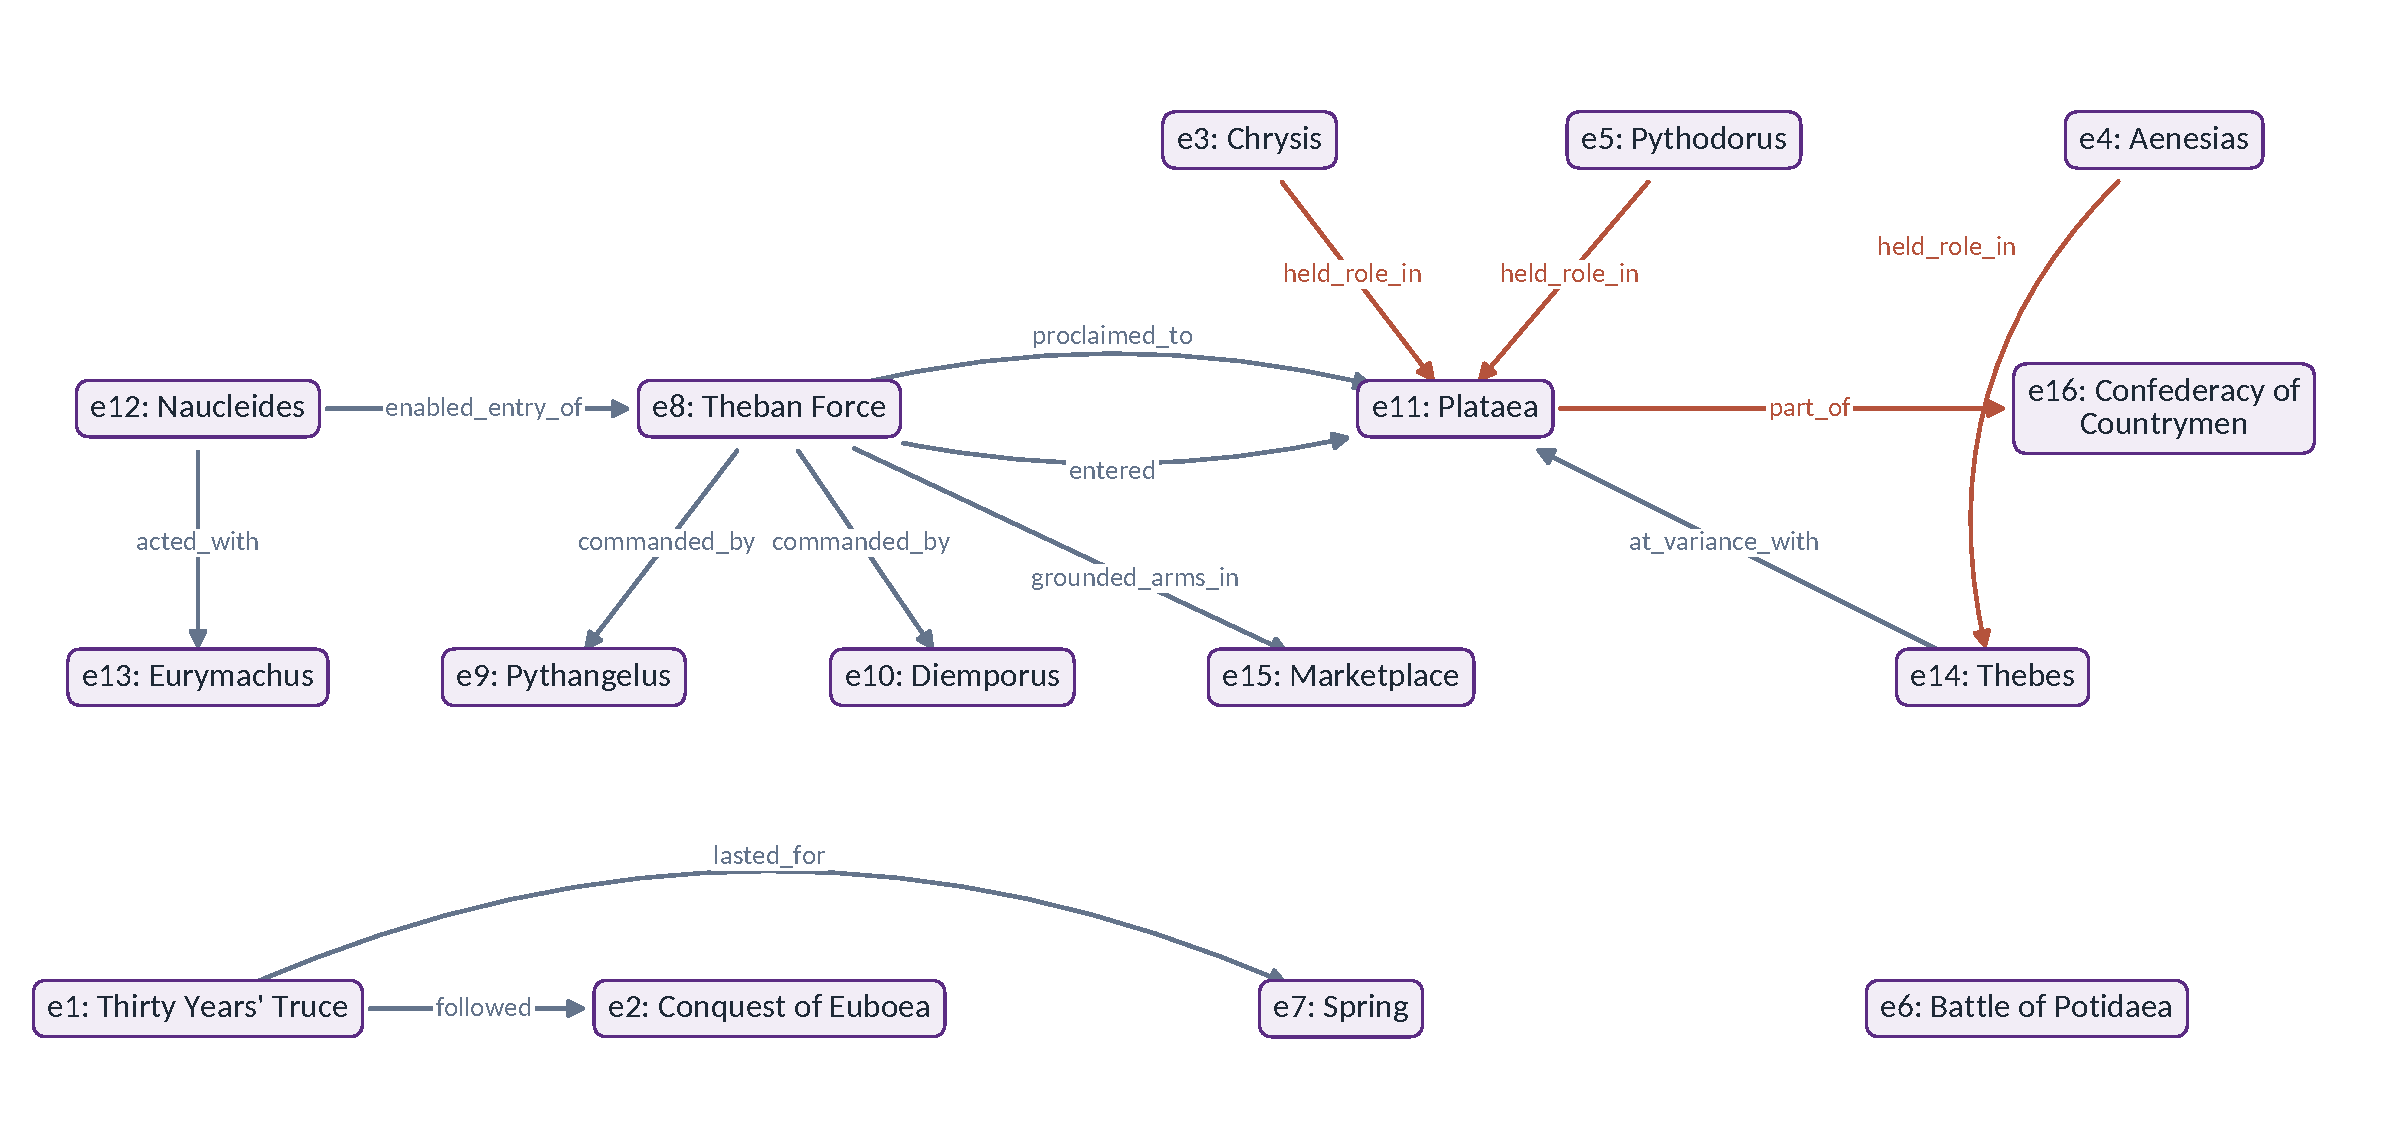
\includegraphics[width=\textwidth,height=.55\textheight,keepaspectratio]{zeugma_materials/full_graph.pdf}\par}
  \footnotesize Orange: the four disputed edges. Other assertions are preserved without certifying them. The isolated Battle of Potidaea entity is retained.
  \source{Drawn from the complete returned entity/relation arrays, 16 September.\newline
  Text, graph, all IDs, literal properties, queries and answers are together in \texttt{zeugma\_materials.pdf}.}
\end{frame}

\begin{frame}{Instructor reference: what was actually tested}
  \small
  \begin{tabular}{@{}lr@{\hspace{2em}}lr@{}}
    \toprule
    \textbf{Run} & \textbf{Seconds} & \textbf{Run} & \textbf{Seconds}\\
    \midrule
    Standard & 7.06 & NeSy3 & 18.85\\
    Cairns & 12.26 & NeSy4 & 60.38\\
    NeSy1 & 24.64 & Zeugma, full & 9.61\\
    NeSy2 & 18.19 & Zeugma, shorter & 10.40\\
    \bottomrule
  \end{tabular}
  \medskip
  \begin{itemize}
    \item Existing live APIs, same English emotion passage, one run per mode.
    \item Logs: 23 successful GPT-4o calls, including feedback and dialogue.
    \item Monitored account-window token cost: approximately \textbf{US\$0.29} before cache discount, below the US\$3 rehearsal allowance.
    \item Browser walkthrough, Greek input and 30-person concurrency remain untested.
    \item No deployment, key configuration or app change.
  \end{itemize}
  \source{Evidence: \texttt{medea\_rehearsal\_report.md} and its linked JSON records.\\
  Times include network and processing. Cost is an account-window calculation, not an invoice or exact per-request charge.}
\end{frame}
\begin{frame}{Nature exercise: full Greek passage, 1 of 3}
\normalsize\raggedright\setlength{\parskip}{5pt}
Όταν η Ελένη επέστρεψε στο χωριό, ο δρόμος προς το λιμάνι μύριζε βρεγμένο χώμα. Τα αλμυρίκια έγερναν πάνω από την άμμο και ένας γλάρος στεκόταν στην άκρη του μόλου. Ο νοτιάς έφερνε μικρά κύματα ως τα σκαλοπάτια των σπιτιών. Πίσω από τις αυλές, τα πεύκα κρατούσαν ακόμη τις σταγόνες της νυχτερινής βροχής. Τίποτε δεν έμοιαζε έκτακτο, κι όμως εκείνη σταμάτησε σαν να έβλεπε τον τόπο πρώτη φορά.

Στο κοινοτικό γραφείο, η υπάλληλος της ζήτησε την ταυτότητά της και τον αριθμό της αίτησης. Η Ελένη περίμενε ώσπου να τελειώσει ένα τηλεφώνημα. Έπειτα παρέλαβε δύο αντίγραφα της απόφασης, υπέγραψε στο σχετικό βιβλίο και ρώτησε πότε είχε εγκριθεί η σύμβαση. Η υπάλληλος της έδειξε την ημερομηνία. Το όνομα του πατέρα της δεν υπήρχε στον κατάλογο των ιδιοκτητών, παρόλο που εμφανιζόταν στο παλαιότερο συμβόλαιο.
\source{Original fictional text written for the workshop. Read all three pages as one passage, keeping the paragraph breaks.\newline Copyable file: \texttt{nature\_excerpt.txt}. Whole Text tested with Claude Sonnet 5, 20 September 2026.}
\end{frame}

\begin{frame}{Nature exercise: full Greek passage, 2 of 3}
\normalsize\raggedright\setlength{\parskip}{5pt}
Στο καφενείο, η απόφαση είχε σηκώσει θύελλα αντιδράσεων. Ένα κύμα διαμαρτυρίας περνούσε από τραπέζι σε τραπέζι, αλλά κανείς δεν συμφωνούσε για το επόμενο βήμα. Ο αδελφός της έλεγε πως το πρόβλημα είχε βαθιές ρίζες και πως οι υποσχέσεις του προέδρου ήταν μόνο καπνός. Εκείνη άκουγε χωρίς να μιλά. Όταν κάποιος τη ρώτησε αν θα προσέφευγε στο δικαστήριο, απάντησε ότι ήθελε πρώτα να διαβάσει τα έγγραφα.

Το απόγευμα κατέβηκε ξανά στην ακτή. Η θάλασσα την περίμενε θυμωμένη και χτυπούσε επίμονα την κλειστή πόρτα μιας αποθήκης. Στο ρέμα δεν υπήρχαν πια καλάμια. Ο πατέρας της έγραφε στο ημερολόγιό του ότι τις ανοιξιάτικες νύχτες δεν μπορούσε να κοιμηθεί από τα βατράχια. Τώρα ακουγόταν μόνο η αντλία του εργοταξίου. Η Ελένη έψαξε με το βλέμμα τις όχθες, χωρίς να ξέρει αν περίμενε να βρει κάτι ή να επιβεβαιώσει την απουσία του.
\source{Original fictional text written for the workshop. Read all three pages as one passage, keeping the paragraph breaks.\newline Copyable file: \texttt{nature\_excerpt.txt}. Whole Text tested with Claude Sonnet 5, 20 September 2026.}
\end{frame}

\begin{frame}{Nature exercise: full Greek passage, 3 of 3}
\normalsize\raggedright\setlength{\parskip}{5pt}
Από το ξωκλήσι ακούστηκε η καμπάνα και μια ηλικιωμένη γυναίκα σταυροκοπήθηκε. Λίγο πιο πέρα, ένας εργάτης έδενε κόκκινες κορδέλες στους κορμούς των ελιών που θα κόβονταν για να περάσει ο νέος δρόμος. Η Ελένη θυμήθηκε τη μητέρα της να απλώνει τα δίχτυα για τη συγκομιδή και να παραπονιέται για τη μικρή σοδειά. Για την ίδια, εκείνα τα δέντρα ήταν μαζί δουλειά, περιουσία και μνήμη. Δεν ήξερε ποια από τις τρεις λέξεις θα χωρούσε στην ένσταση.
\source{Original fictional text written for the workshop. Read all three pages as one passage, keeping the paragraph breaks.\newline Copyable file: \texttt{nature\_excerpt.txt}. Whole Text tested with Claude Sonnet 5, 20 September 2026.}
\end{frame}

\end{document}
